
\documentclass[
	11pt, 
]{beamer}

\graphicspath{{Images/}{./}}

\usepackage{booktabs}
\usetheme{Madrid}
\usefonttheme{default}
\usepackage{palatino}
\usepackage[default]{opensans}
\useinnertheme{circles}
\setbeamertemplate{caption}[numbered]
%----------------------------------------------------------------------------------------
%	PRESENTATION INFORMATION
%----------------------------------------------------------------------------------------

\title{Extreme Programming}

\subtitle{CSMI1}
\author[S.KARAMI \and SABA \and ADIENG \and WADE]{P. S.KARAMI \and O. SABA \and A. DIENG \and A. WADE}
\institute[]{University of Strasbourg \\ \smallskip} % Your institution, the optional parameter can be used for the institution shorthand and will appear on the bottom of every slide after author names, while the required parameter is used on the title slide and can include your email address or additional information on separate lines

\date[\today]{Mathematics and applications \\ \today} % Presentation date or conference/meeting name, the optional parameter can contain a shortened version to appear on the bottom of every slide, while the required parameter value is output to the title slide

%----------------------------------------------------------------------------------------

\begin{document}

%----------------------------------------------------------------------------------------
%	TITLE SLIDE
%----------------------------------------------------------------------------------------

\begin{frame}
	\titlepage % Output the title slide, automatically created using the text entered in the PRESENTATION INFORMATION block above
\end{frame}

%----------------------------------------------------------------------------------------
%	TABLE OF CONTENTS SLIDE
%----------------------------------------------------------------------------------------

\begin{frame}
	\frametitle{Presentation Overview} % Slide title, remove this command for no title
	
	\tableofcontents 
\end{frame}

%----------------------------------------------------------------------------------------
%	PRESENTATION BODY SLIDES
%----------------------------------------------------------------------------------------

\section{Introduction}

%------------------------------------------------

\subsection{Definition}

\begin{frame}
	\frametitle{Definition}
	
	Extreme programming (XP) has been designed and developed to meet the specific needs of software development by small teams with vague and changing requierements.	
	\bigskip % Vertical whitespace
	\begin{figure}
		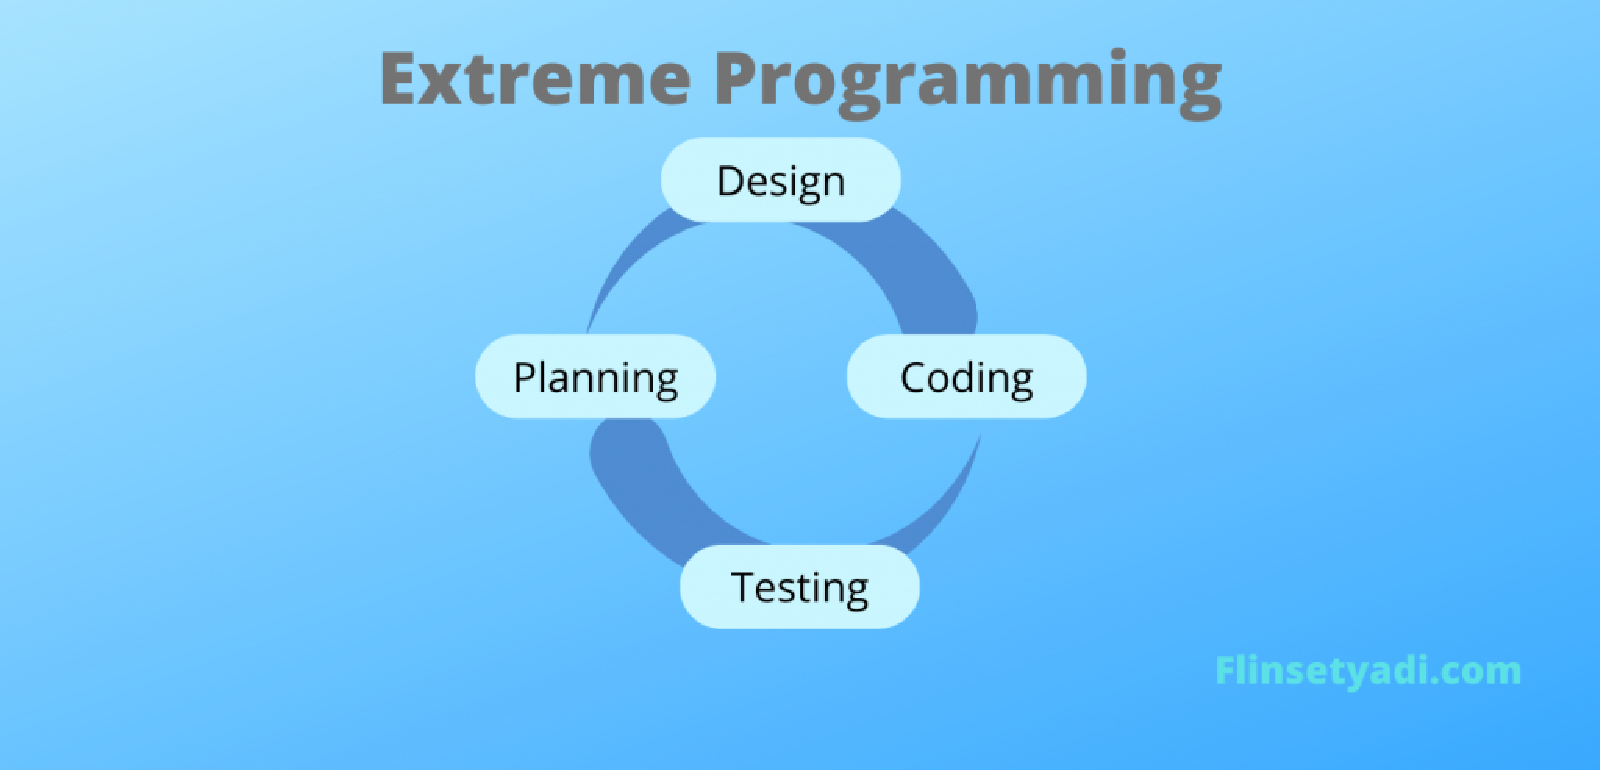
\includegraphics[width=0.8\linewidth]{ext2.pdf}
		\caption{Extreme programming\cite{p1}}
	\end{figure}

\end{frame}

%------------------------------------------------
\subsection{Applications}

\begin{frame}
	\frametitle{Applications}
		Xp is one of the Agile software development methoddologies applied by IT
companies. It provides values and principles to guide the behaviour of the team.
The team is expected to be self-organizing core practices where:
	\begin{enumerate}
		\item Each practice is simple and self-completing;
		\item The combination of practices produces more complex and emergent behaviour. 
	\end{enumerate}
	\bigskip % Vertical whitespace

\end{frame}
%---------------------------------------------------------------------------------------
%------------------------------------------------

\section{Methodology}
\subsection{How Does Extreme Programming (XP) Work}
\begin{frame}
	\frametitle{How Does Extreme Programming (XP) Work?}
	How Does Extreme Programming (XP) Work?
	\bigskip % Vertical whitespace
	\begin{figure}
		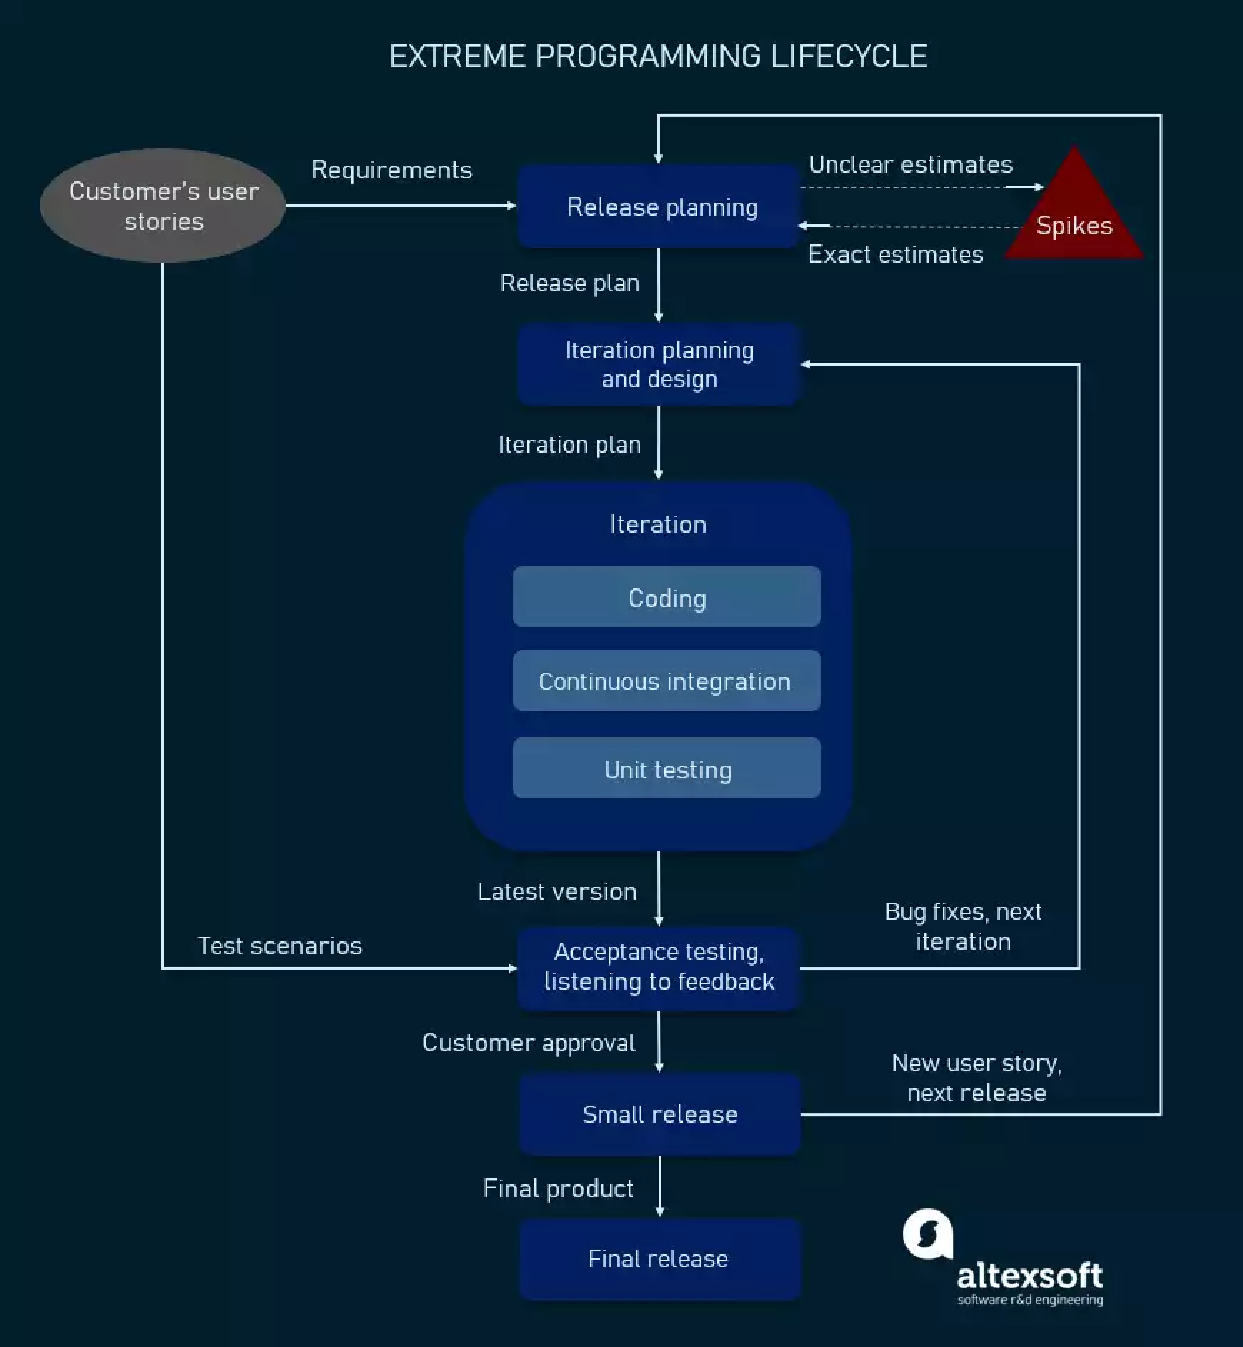
\includegraphics[width=0.475\linewidth]{ext3.pdf}
		\caption{Extreme programming \cite{p5}}
	\end{figure}
\end{frame}
%------------------------------------------------------------------------
\begin{frame}
	\frametitle{How Does Extreme Programming (XP) Work}
	\begin{figure}
		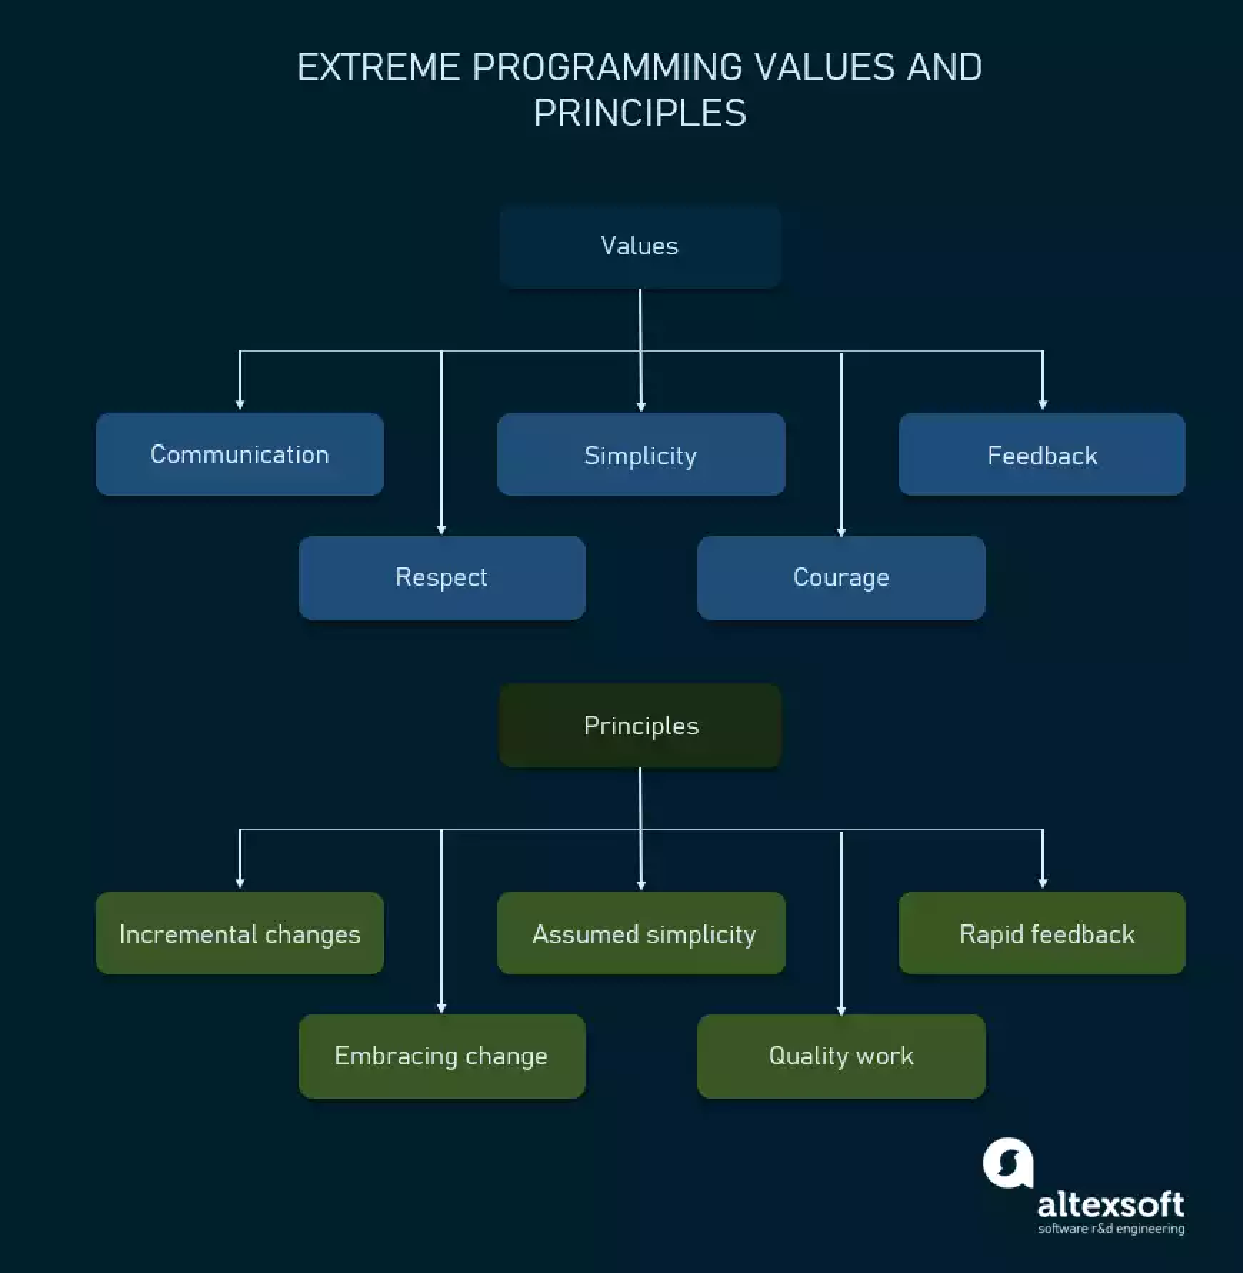
\includegraphics[width=0.55\linewidth]{ext4.pdf}
		\caption{Extreme programming \cite{p5}}
	\end{figure}
\end{frame}
%------------------------------------------------
\subsection{Advantages and disadvantages}
\begin{frame}
	\frametitle{Advantages and disadvantages}
The main advantage of Extreme Programming is that this methodology allows
software development companies to save costs and time required for project
realization.
Simplicity : the XP developers create extremely simple code that can be
improved at any moment.
Constant feedback is also the strong side.It is necessary to listen and make
any changes needed in time.\cite{p1,p4}
	\bigskip % Vertical whitespace
\end{frame}
%--------------------------------------------------------------------------------
\begin{frame}
	\frametitle{Advantages and disadvantages}
	\begin{figure}
		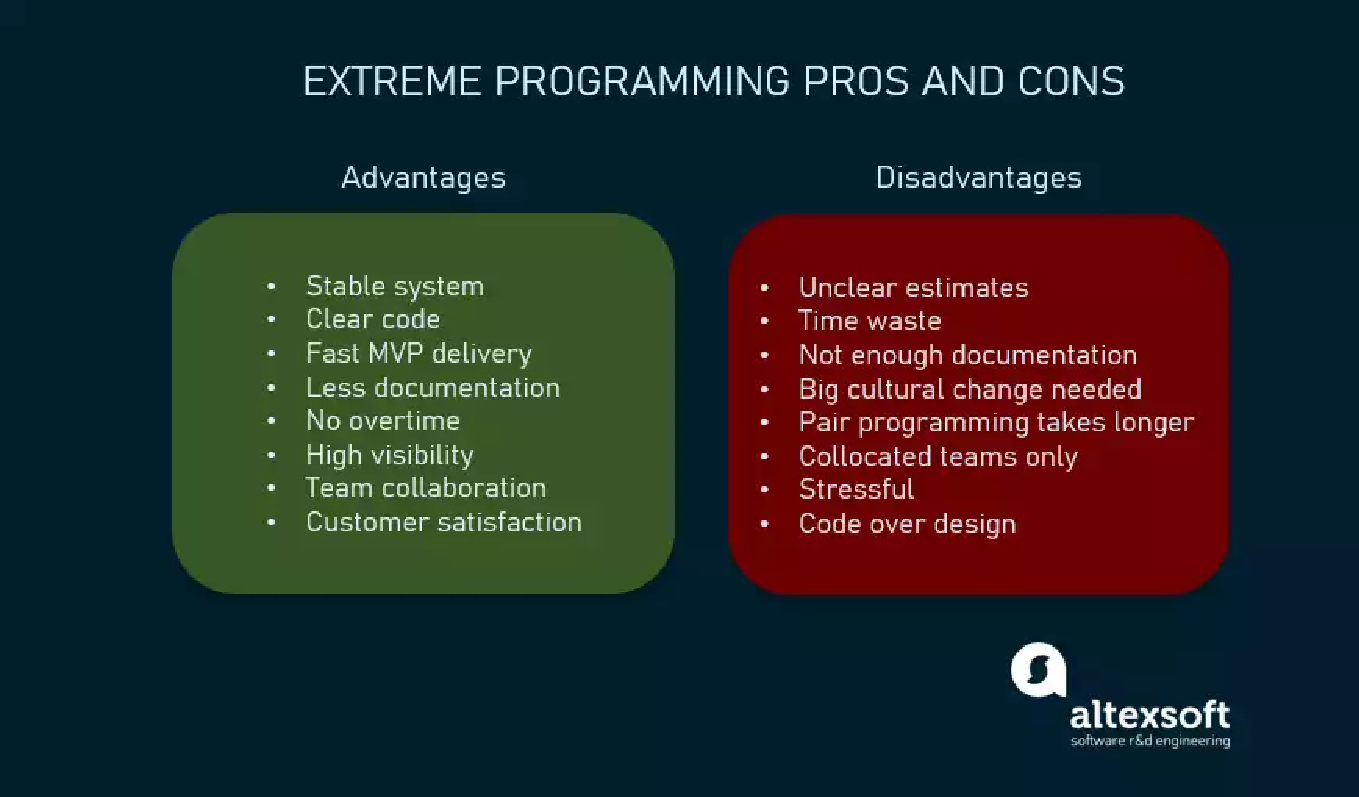
\includegraphics[width=0.8\linewidth]{ext5.pdf}
		\caption{Table of advantages and disadvantages \cite{p4}}
	\end{figure}
\end{frame}
%---------------------------------------------------------------------------------
\subsection{Comparison of XP with other frameworks}
\begin{frame}
	\frametitle{Comparison of XP with other frameworks}
	\begin{figure}
		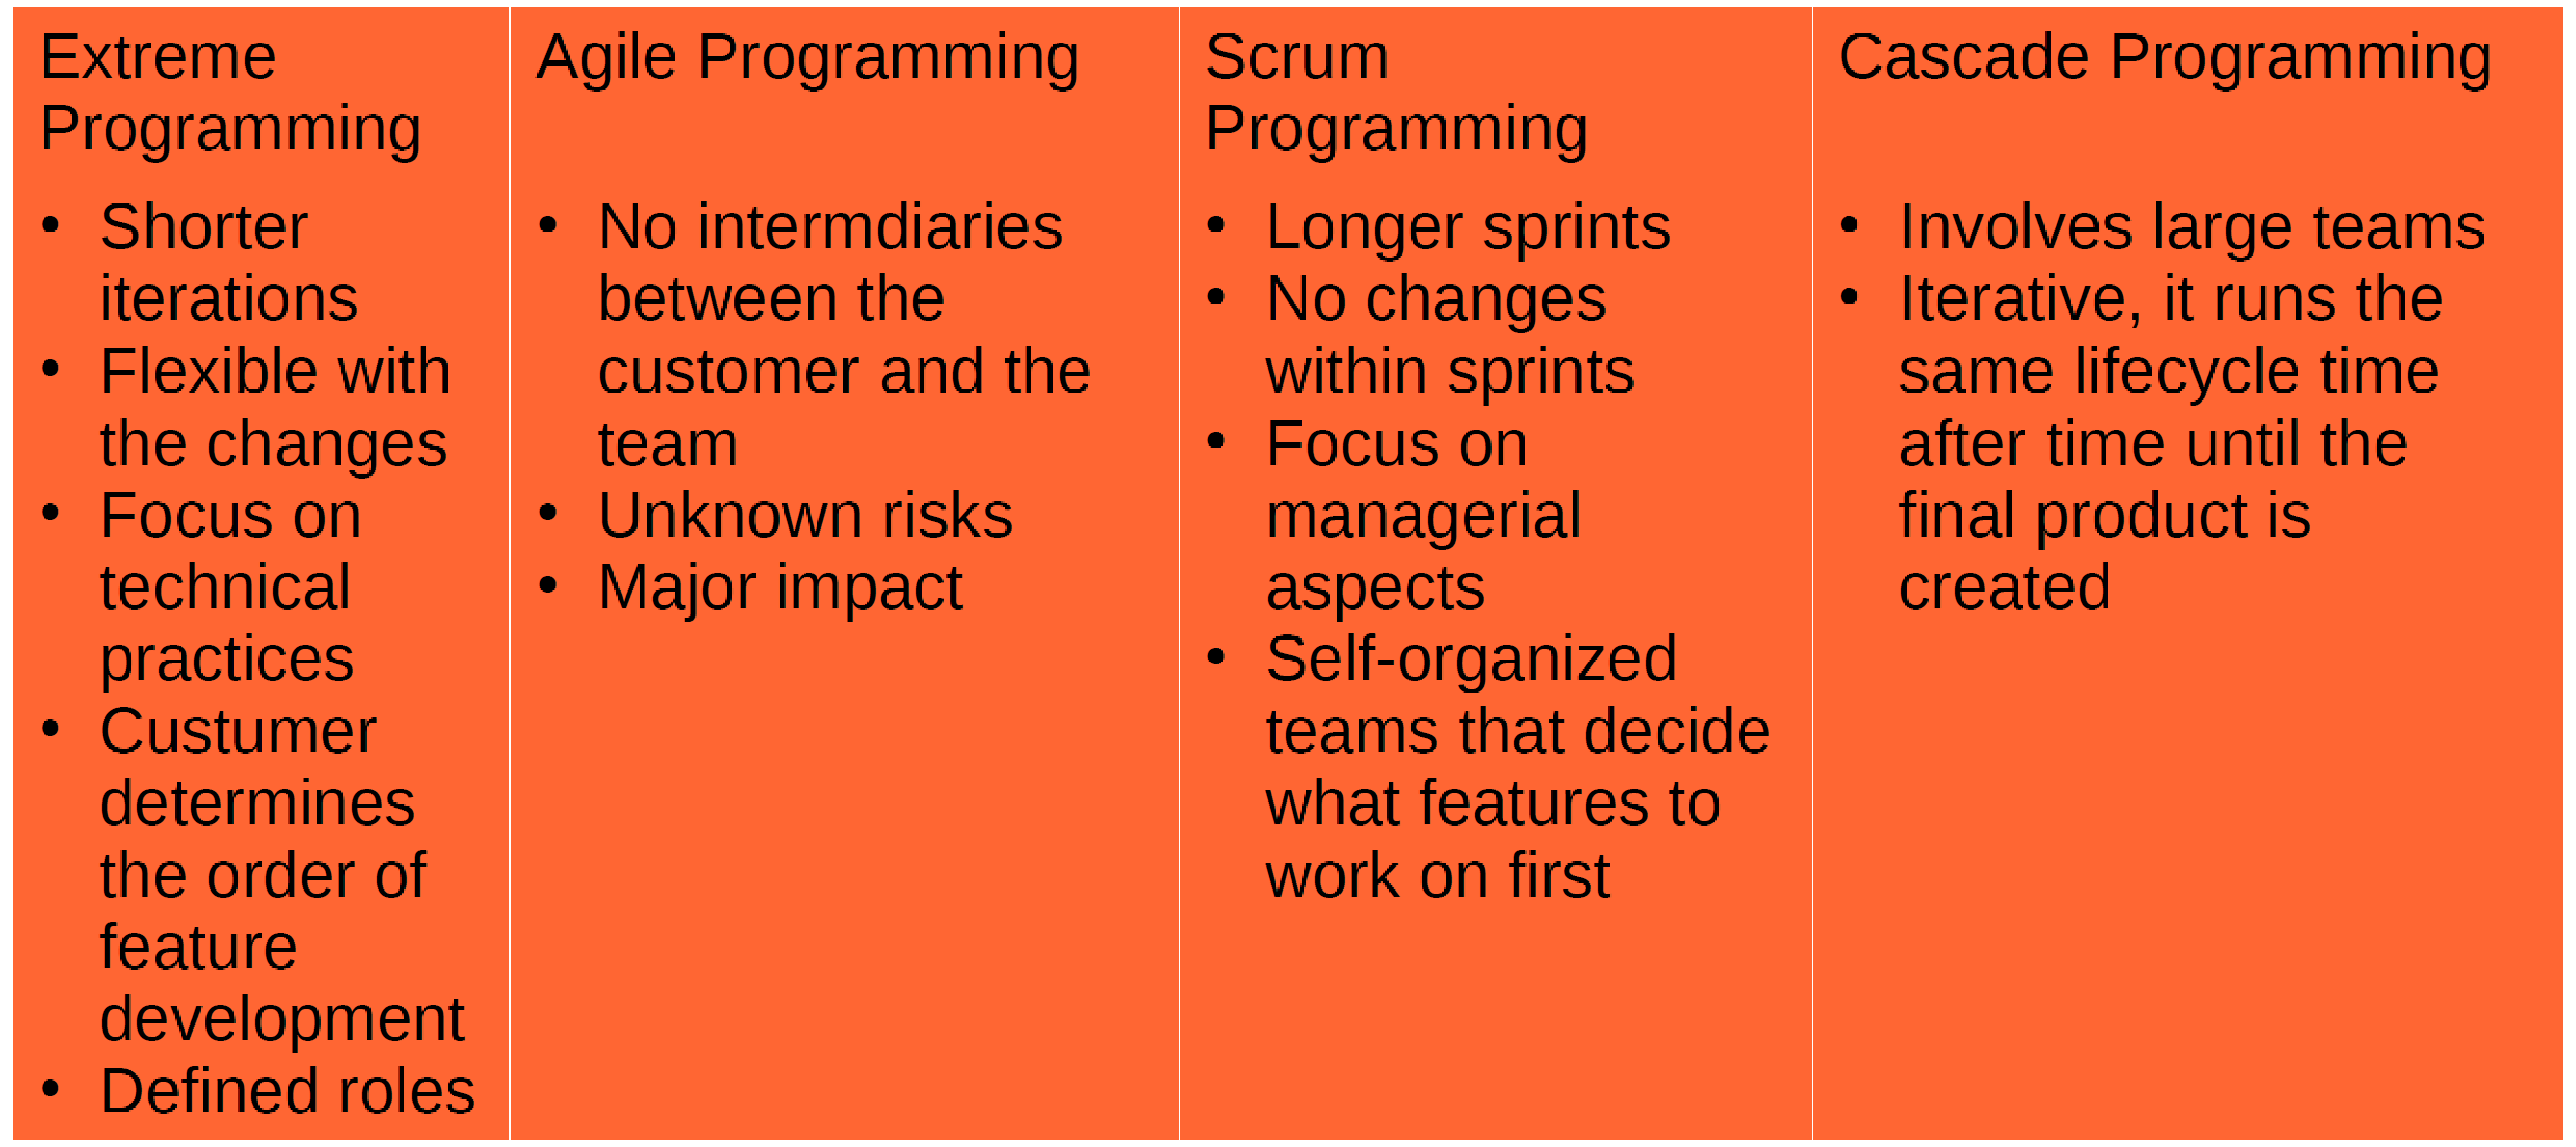
\includegraphics[width=0.8\linewidth]{ext6.pdf}
		\caption{Comparison of XP with other frameworks \cite{p2}}
	\end{figure}
	\bigskip % Vertical whitespace
\end{frame}
%---------------------------------------------------------------------------------
\section{Conclusion}
\subsection{Conclusion}
\begin{frame}
	\frametitle{Conclusion}
	There is no such thing as the best methodology. Project Managers must weigh project aspects against available methodologies to make an
appropriate selection. If a certain development process has been working well then it will be wise to stick with it. Other methodologies like XP,
Scrum, Argile or Waterfall can be reviewed to borrow some good and applicable ideas into the current methodology in use.\cite{p7,p8}
	\bigskip % Vertical whitespace
\end{frame}
%-----------------------------------------------------------------------------------
\section{References}
\begin{frame} % Use [allowframebreaks] to allow automatic splitting across slides if the content is too long
	\frametitle{References}
	
	\begin{thebibliography}{99} % Beamer does not support BibTeX so references must be inserted manually as below, you may need to use multiple columns and/or reduce the font size further if you have many references
		\footnotesize % Reduce the font size in the bibliography
		
		\bibitem[1]{p1}
		 www.wrytradesman.com/articles/IntroToAgileMethods.pdf
		\bibitem[2]{p2}
		www.extremeprogramming.org
		\bibitem[3]{p3}
		www.xprogramming.com/xpmag/whatisxp.htm
		\bibitem[4]{p4}
		www.selectbs.com/glossary/what-is-extreme-programming.htm
		\bibitem[5]{p5}
		https://www.altexsoft.com/blog/business/extreme-programming-values-principles-and-practices/
		\bibitem[6]{p6}
			 Kenneth E. Kendall (2004)
			\newblock Programmation extrême en pratique : Une approche à valeure humaine du système de gestion
de conférence DSI , Ligne de décision Vol. 35

		\bibitem[7]{p7}
			Scott Withrow
			\newblock Extreme Programming : Ces 12 pratiques rendent-elles parfaites
http://articles.techrepublic.com.com/5100-22-11-1046488.html

		\bibitem[8]{p8}
			 B. Rumpe , P. Scholz
			\newblock Mise à l' échelle de la gestion des projets de programmation extrême , Projets et bénéfices
Numéro spécial sur la gestion des projets de programmation extrême, Vol. III (8), p. 11-18. ICFAI Press, Hyderabat ,
août 2003.
	\end{thebibliography}
\end{frame}
%----------------------------------------------------------------------------------------
%	CLOSING SLIDE
%----------------------------------------------------------------------------------------

\begin{frame}[plain] % The optional argument 'plain' hides the headline and footline
	\begin{center}
		{\Huge The End}
		
		\bigskip\bigskip % Vertical whitespace
		
		{\LARGE Questions? Comments?}
	\end{center}
\end{frame}

%----------------------------------------------------------------------------------------

\end{document} 